\documentclass[pdflatex,compress,mathserif]{beamer}

%\usetheme[dark,framenumber,totalframenumber]{ElektroITK}
\usetheme[darktitle,framenumber,totalframenumber]{ElektroITK}

\usepackage[utf8]{inputenc}
\usepackage[T1]{fontenc}
\usepackage{lmodern}
\usepackage[bahasai]{babel}
\usepackage{amsmath}
\usepackage{amsfonts}
\usepackage{amssymb}
\usepackage{graphicx}
\usepackage{multicol}
\usepackage{lipsum}
\usepackage{framed}
\usefonttheme[onlymath]{serif}

\newcommand*{\Scale}[2][4]{\scalebox{#1}{$#2$}}%

\setbeamertemplate{caption}[numbered]

\title{PENGOLAHAN SINYAL DIGITAL}
\subtitle{Proses Sampling}

\author{Mifta Nur Farid}

\begin{document}

\maketitle

\begin{frame}{Diagram blok pengolahan\\sinyal digital}
    \begin{figure}
        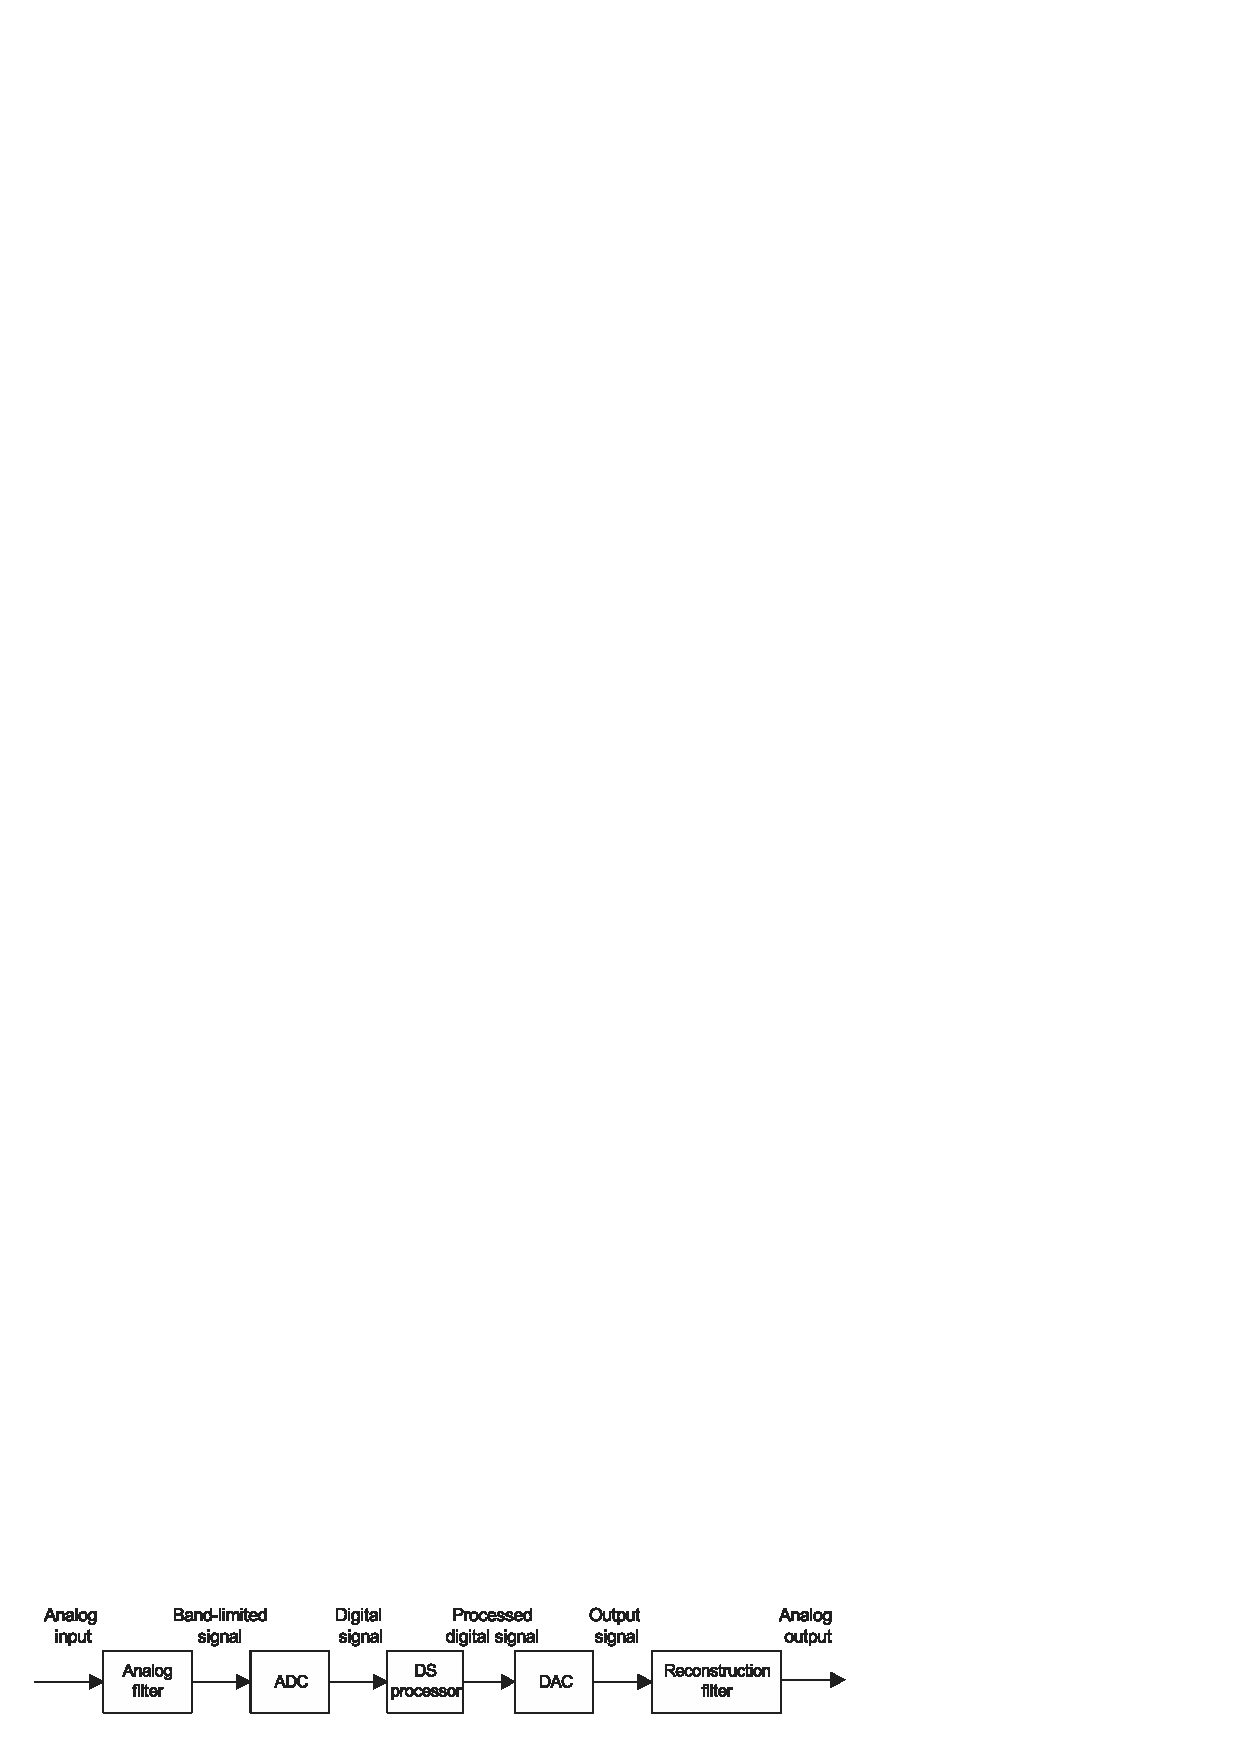
\includegraphics[width=\linewidth]{./img/img01.png}
    \end{figure}
\end{frame}

\begin{frame}{Proses sampling dalam domain\\waktu}
    \begin{itemize}
        \item Sinyal waktu kontinyu memiliki titik yang tak berhingga
        \item Tidak mungkin mendigitalkan titik yang tak berhingga karena membutuhkan banyak memory dalam komputasinya
        \item Solusinya $\rightarrow$ sampling $\rightarrow$ T = sampling interval atau sampling period (detik)
        \begin{figure}
            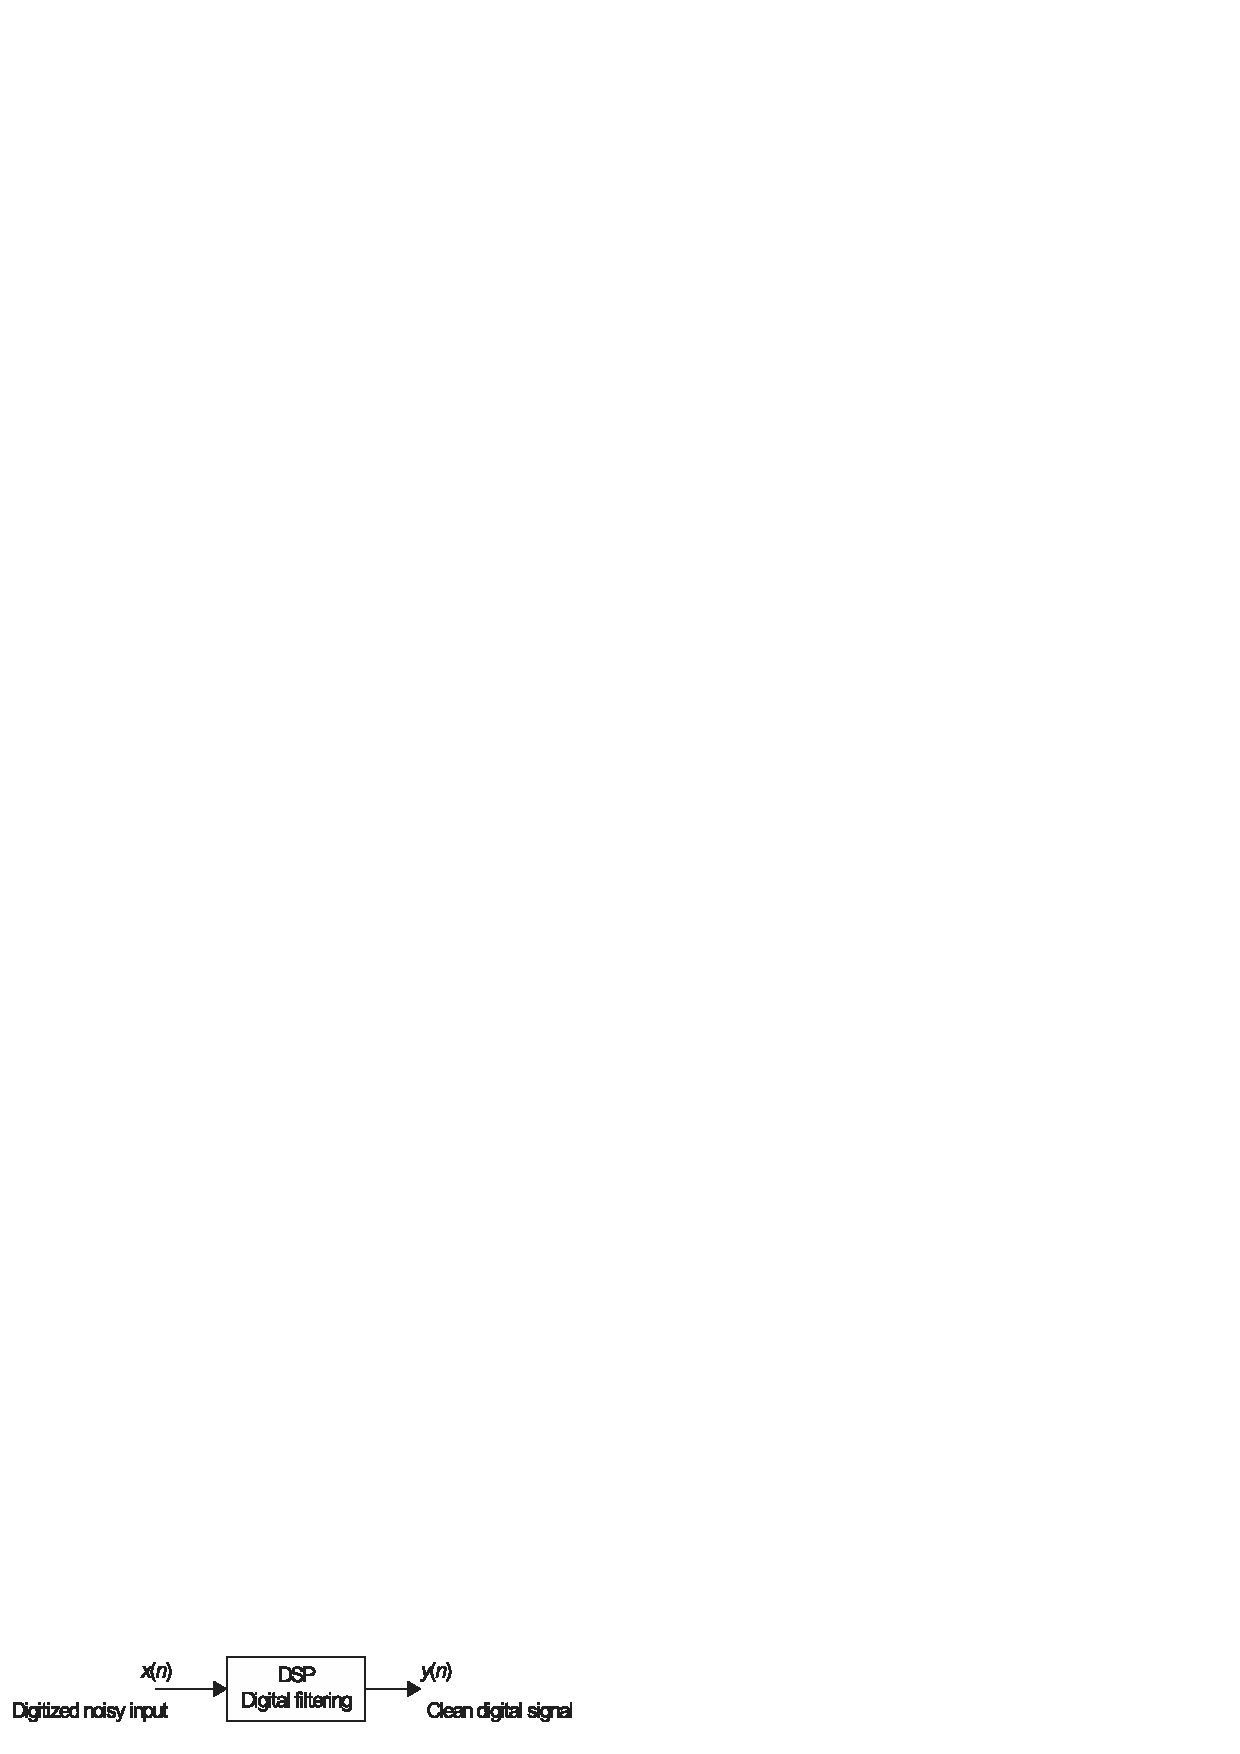
\includegraphics[width=0.9\linewidth]{./img/img02.png}
        \end{figure}
    \end{itemize}
\end{frame}

\begin{frame}{Sample-and-hold tegangan analog\\untuk ADC}
    \begin{itemize}
        \item Setiap sample mempertahankan nilai tegangannya selama interval $T$ $\rightarrow$ memberikan cukup waktu untuk ADC mengubahnya
        \item Metode sampling: \textbf{Sample-and-Hold}
        \begin{figure}
            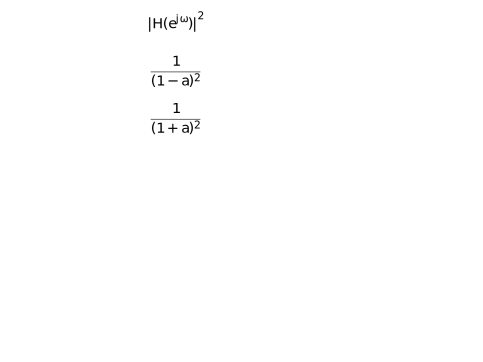
\includegraphics[width=0.9\linewidth]{./img/img03.png}
        \end{figure}
    \end{itemize}
\end{frame}

\begin{frame}{Sampling rate}
    \begin{itemize}
        \item Untuk setiap sampling interval $T$ yang diberikan, sampling rate $f_s$ adalah
        \begin{equation}
            f_s = \frac{1}{T} \text{ samples per second (Hz)}
        \end{equation}
        \item Contoh: jika sampling period, $T$, adalah 125 $\mu s$, maka sampling rate adalah $$ f_s = \frac{1}{125 \mu s} = 8000 \text{ Hz} $$
    \end{itemize}
\end{frame}

\begin{frame}{Teorema Sampling}
    \begin{itemize}
        \item Berapa minimum sampling rate yang dibutuhkan agar dapat merekonstruksi sinyal analog?
        \item Jika sinyal analog tidak di-sampling dengan baik maka akan terjadi \textbf{aliasing}
    \end{itemize}    
\end{frame}

\begin{frame}{Teorema Sampling}
    \begin{figure}
        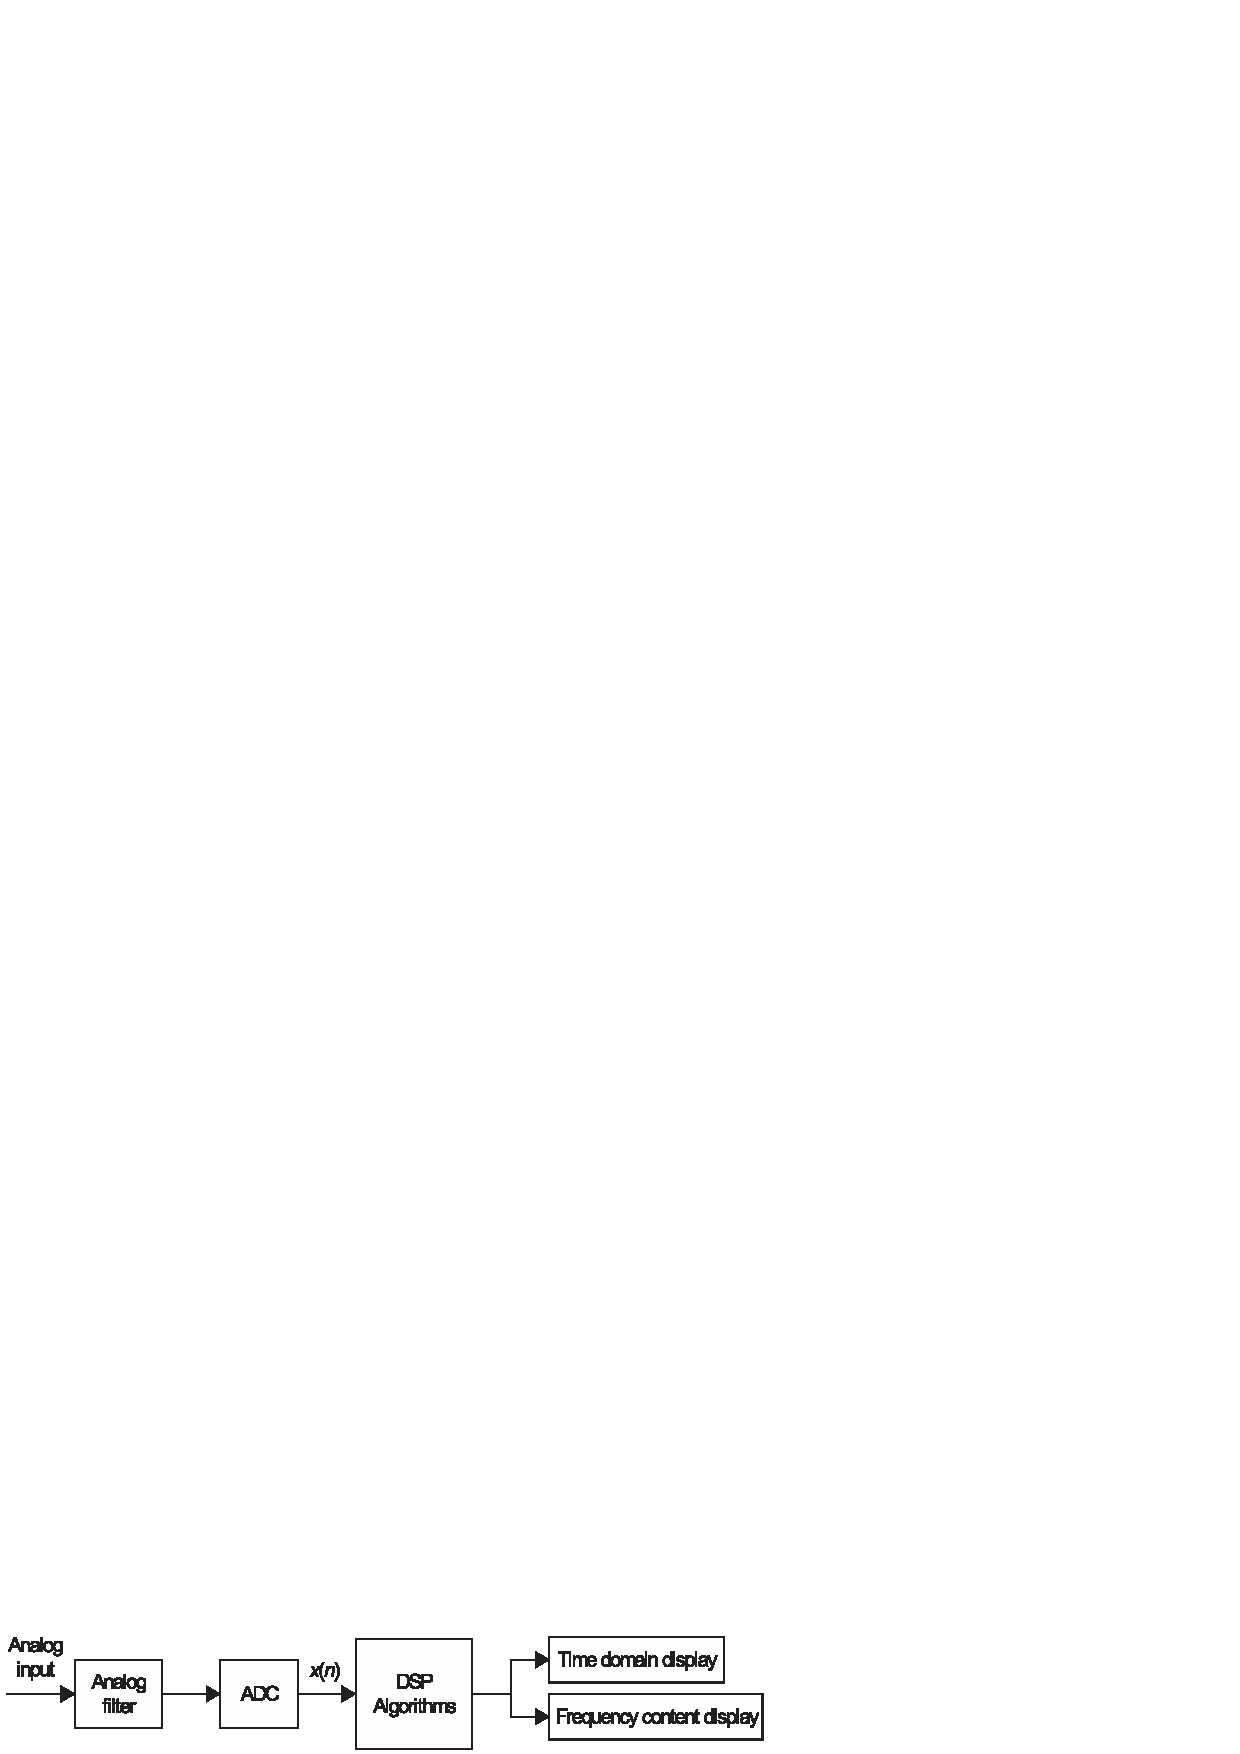
\includegraphics[width=\linewidth]{./img/img04.png}
    \end{figure}
\end{frame}

\begin{frame}{Teorema Sampling}
    \begin{figure}
        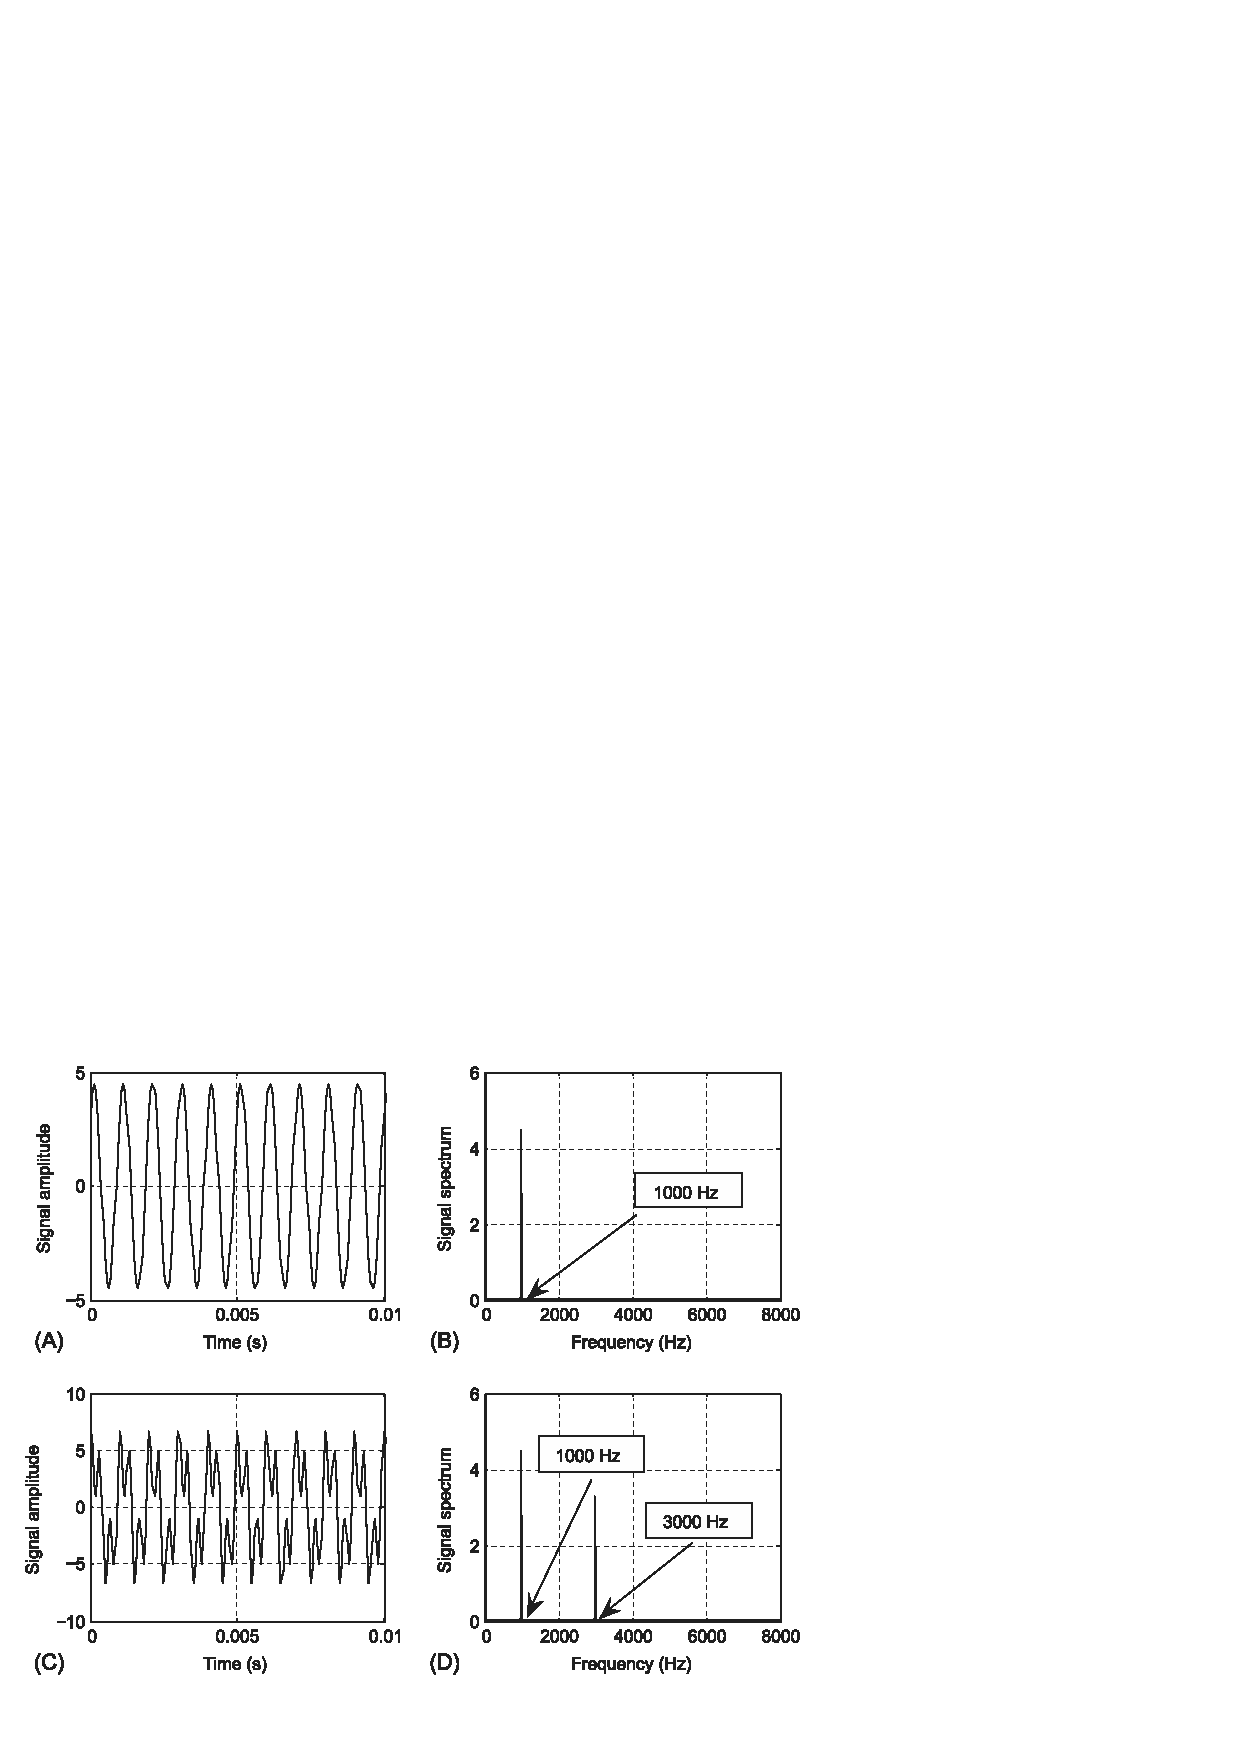
\includegraphics[width=\linewidth]{./img/img05.png}
    \end{figure}
\end{frame}

\begin{frame}{Teorema Sampling}
    \begin{itemize}
        \item Sinyal analog dapat direkonstruksi dengan baik selama sampling rate-nya minimal 2 kali daripada komponen frekuensi tertinggi dari sinyal analognya

        \begin{equation}
            f_s \geq 2 f_\text{max}
        \end{equation}

        $f_\text{max}$ adalah komponen frekuensi tertinggi dari sinyal analog
        \item Contoh: sinyal suara yang mengandung banyak frekuensi hingga 4 kHz, minimum sampling rate yang dipilih setidaknya 8 kHz atau 8000 sampel per detik
    \end{itemize}
\end{frame}

\begin{frame}{Teorema Sampling}
    \begin{itemize}
        \item Berapa sampling rate minimum untuk sinyal analog berikut ini?
        \begin{multicols}{2}
            \begin{enumerate}
                \item[a.] 500 Hz
                \item[b.] 1000 Hz
                \columnbreak
                \item[c.] 1500 Hz
                \item[d.] 2000 Hz
            \end{enumerate}
        \end{multicols}
        \begin{figure}
            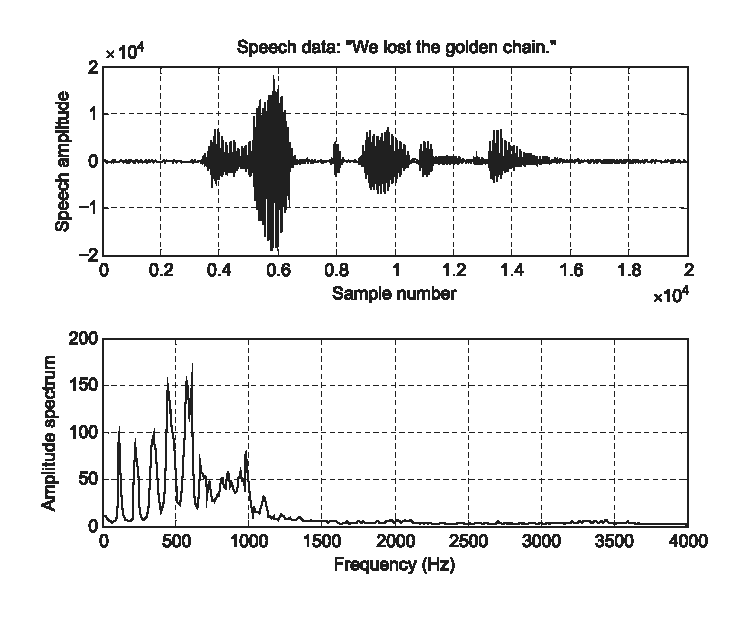
\includegraphics[width=\linewidth]{./img/img06}
        \end{figure}
    \end{itemize}
\end{frame}

\begin{frame}{Teorema Sampling}
    \begin{itemize}
        \item Berapa sampling rate minimum untuk sinyal analog berikut ini?
        \begin{multicols}{2}
            \begin{enumerate}
                \item[a.] 2000 Hz
                \item[b.] 4000 Hz
                \columnbreak
                \item[c.] 6000 Hz
                \item[d.] 8000 Hz
            \end{enumerate}
        \end{multicols}
        \begin{figure}
            \includegraphics[width=\linewidth]{./img/img07}
        \end{figure}
    \end{itemize}
\end{frame}

\begin{frame}{Teorema Sampling}
    \begin{figure}
        \includegraphics[width=0.9\linewidth]{./img/img08}
    \end{figure}
\end{frame}

\begin{frame}{Teorema Sampling}
    \begin{itemize}
        \item Proses sampling
        \begin{equation}
            x_s(t) = x(t) p(t)
            \label{eq:xs}
        \end{equation}
        yang mana $p(t)$ adalah pulse train dengan period $T = \frac{1}{f_s}$
        \item Pulse train:
        \begin{equation}
            p(t) = \sum_{n = - \infty}^\infty \delta(t - nT)
        \end{equation}
    \end{itemize}
\end{frame}

\begin{frame}{Teorema Sampling}
    \begin{itemize}
        \item Dengan frekuensi dasar, $\omega_0 = 2\pi/T = 2\pi f_s$ rad/s, $p(t)$ dapat direpresentasikan dalam bentuk deret Fourier
        \begin{equation}
            p(t) = \sum_{k = - \infty}^\infty a_k e^{jk\omega_0t}
            \label{eq:pt_deret}
        \end{equation}
        yang mana $a_k$ adalah koef. Fourier yang dapat ditentukan oleh
        \begin{equation}
            a_k = \frac{1}{T} \int_{-\infty}^{\infty} \delta(t)e^{-jk\omega_0t}dt = \frac{1}{T}
            \label{eq:keof.Fourier}
        \end{equation}
    \end{itemize}
\end{frame}

\begin{frame}{Teorema Sampling}
    \begin{itemize}
        \item Substitusikan Pers. (\ref{eq:keof.Fourier}) ke Pers. (\ref{eq:pt_deret}), didapatkan
        \begin{equation}
            p(t) = \sum_{k = -\infty}^{\infty} \frac{1}{T} e^{jk\omega_0t}
            \label{eq:pt_new}
        \end{equation}
        \item Substitusikan Pers. (\ref{eq:pt_new}) ke Pers. (\ref{eq:xs}), didapatkan
        \begin{equation}
            x_s(t) = \sum_{k = -\infty}^{\infty} \frac{1}{T} x(t) e^{jk\omega_0t}
            \label{eq:xs_new}
        \end{equation}
    \end{itemize}
\end{frame}

\begin{frame}{Teorema Sampling}
    \begin{itemize}
        \item Transformasi Fourier dari Pers. (\ref{eq:xs_new}):
        \begin{align}
            X_s(f) &= \text{FT} \left\{ \sum_{k = -\infty}^{\infty} \frac{1}{T} x(t) e^{jk\omega_0t} \right\} \\
            &= \sum_{k = -\infty}^{\infty} \frac{1}{T} \text{ FT} \left\{ x(t) e^{jk\omega_0t} \right\} \\
            &= \sum_{k = -\infty}^{\infty} \frac{1}{T} \int_{-\infty}^{\infty} \left\{ x(t) e^{jk\omega_0t} \right\}e^{-j\omega t} dt\\
            &= \sum_{k = -\infty}^{\infty} \frac{1}{T} \int_{-\infty}^{\infty} x(t) e^{-j(\omega-k\omega_0) t} dt \\
            X_s(f) &= \sum_{k = -\infty}^{\infty} \frac{1}{T} \int_{-\infty}^{\infty} x(t) e^{-j2\pi(f-kf_s) t} dt
            \label{eq:Xsf}
        \end{align}
    \end{itemize}
\end{frame}

\begin{frame}{Teorema Sampling}
    \begin{itemize}
        \item Berdasarkan definisi dari Transformasi Fourier, kita tahu bahwa
        \begin{equation}
            X(f) = \sum_{k = -\infty}^{\infty} \frac{1}{T} \int_{-\infty}^{\infty} x(t) e^{-j2\pi ft} dt
            \label{eq:Xf}
        \end{equation}
        \item Kita dapatkan hubungan antara Pers. (\ref{eq:Xf}) dan Pers. (\ref{eq:Xsf})
        \begin{equation}
            X_s(f) = \frac{1}{T} \sum_{k = -\infty}^{\infty} X(f - kf_s)
            \label{eq:Xsf_and_Xf}
        \end{equation}
        yang mana $X(f)$ adalah original baseband spectrum sedangkan $X_s(f)$ sampled signal spectrum yang terdiri dari original baseband spectrum $X(f)$ dan kembarannya $X(f\pm kf_s)$
    \end{itemize}
\end{frame}

\begin{frame}{Teorema Sampling}
    \begin{itemize}
        \item Kita lanjutkan Pers. (\ref{eq:Xsf_and_Xf}):
        \begin{equation}
            X_s(f) = \cdots + \frac{1}{T}X(f+f_s) + \frac{1}{T}X(f) + \frac{1}{T}X(f-f_s) + \cdots
            \label{eq:deret_Xsf_and_Xf}
        \end{equation}
        \item sampled signal spectrum merupakan penjumlahan dari scaled original spectrum dan kembarannya (shifted-version of scaled original spectrum)
        \item Pers. (\ref{eq:deret_Xsf_and_Xf}) memiliki kemungkinan 3 grafik berdasarkan nilai sampling rate-nya ($f_s$)
    \end{itemize}
\end{frame}

\begin{frame}{Teorema Sampling}
    \begin{itemize}
        \item Kondisi 1: sampled signal spectrum terpisah dengan kembarannya
        \begin{figure}
            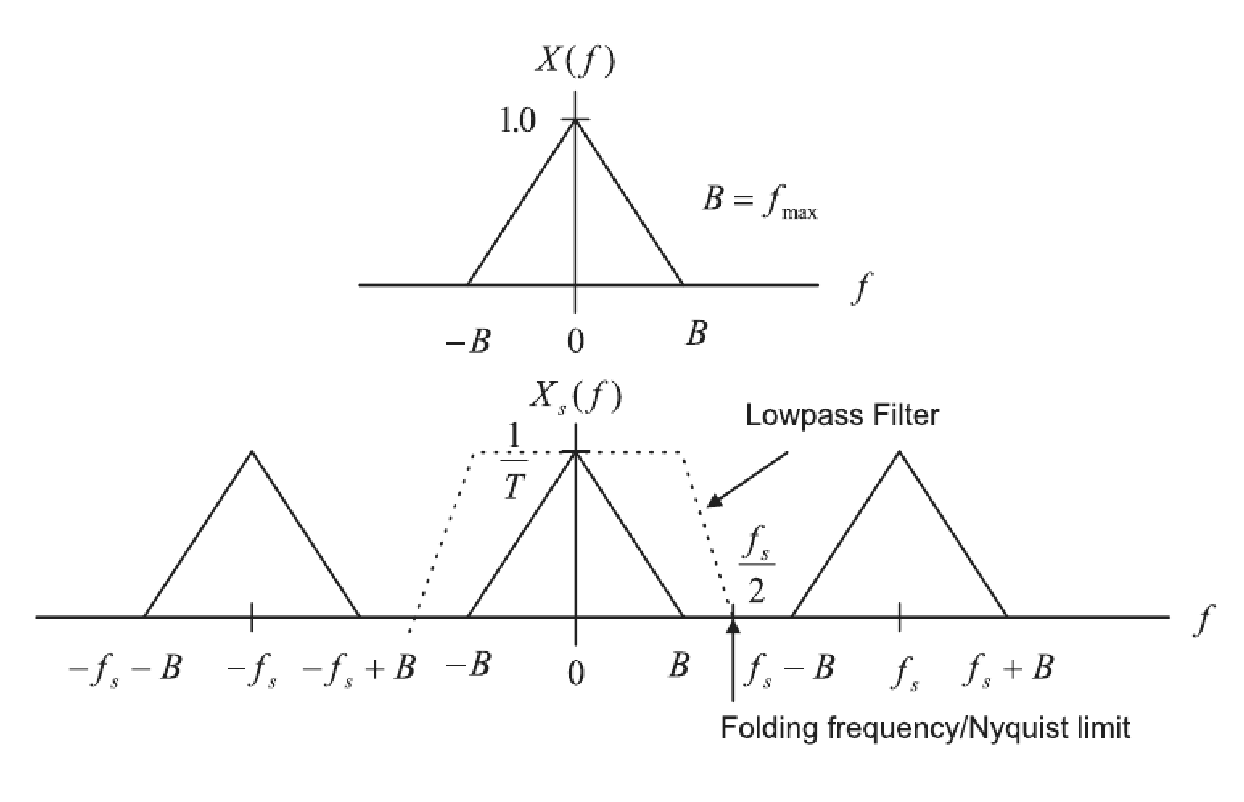
\includegraphics[width=\linewidth]{./img/img09}
            \label{img:09}
        \end{figure}
    \end{itemize}
\end{frame}

\begin{frame}{Teorema Sampling}
    \begin{itemize}
        \item Kondisi 2: sampled signal spectrum terhubung dengan kembarannya
        \begin{figure}
            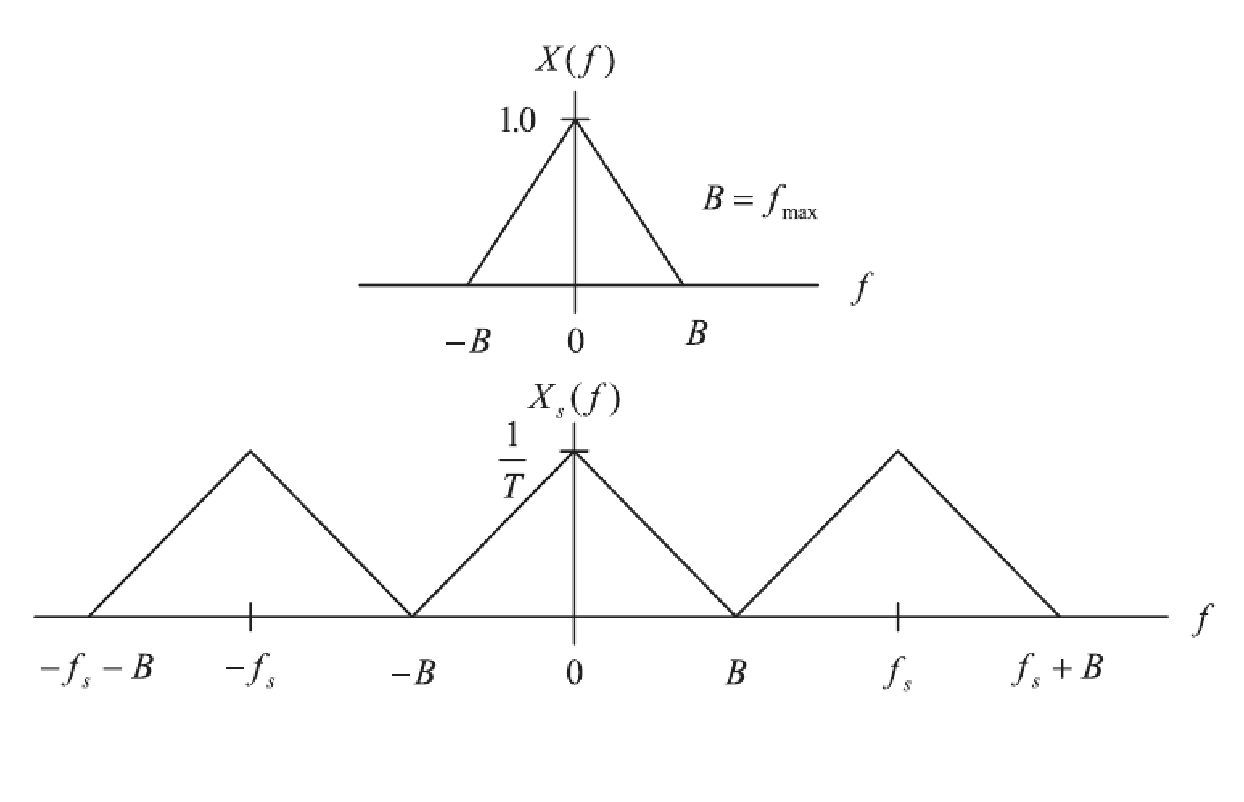
\includegraphics[width=\linewidth]{./img/img10}
        \end{figure}
    \end{itemize}
\end{frame}

\begin{frame}{Teorema Sampling}
    \begin{itemize}
        \item Kondisi 3: sampled signal spectrum overlapped dengan kembarannya
        \begin{figure}
            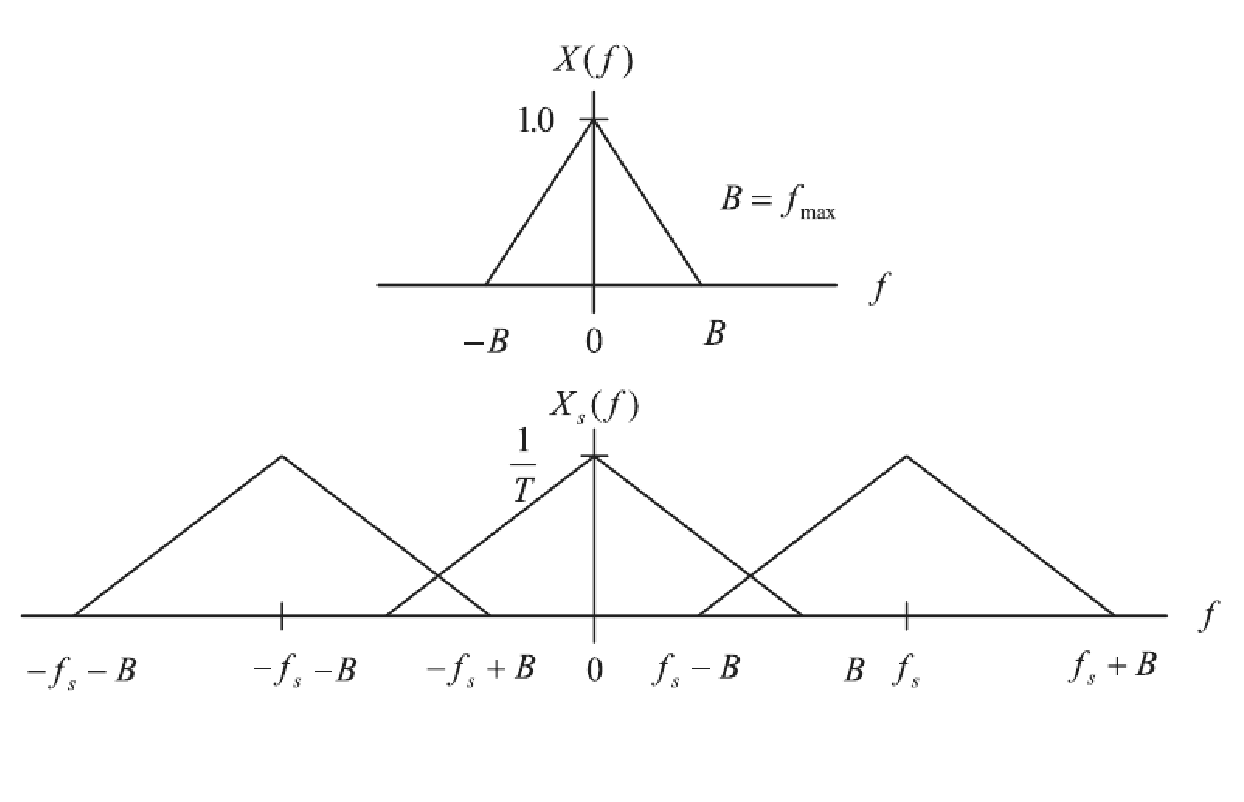
\includegraphics[width=\linewidth]{./img/img11}
        \end{figure}
    \end{itemize}
\end{frame}

\begin{frame}{Teorema Sampling}
    \begin{itemize}
        \item Jika kita gunakan lowpass reconstruction filter untuk mendapatkan hasil rekonstruksi dari original signal spectrum, maka kondisi berikut ini harus terpenuhi:
        \begin{equation}
            f_s - f_{\text{max}} \geq f_{\text{max}}
        \end{equation}
        dengan kata lain
        \begin{equation}
            f_s \geq 2f_{\text{max}}
            \label{eq:freq_nyquist}
        \end{equation}
        atau frekuensi dalam bentuk rad/sec.
        \begin{equation}
            \omega_s \geq 2\omega_{\text{max}}
        \end{equation}
        \item Teorema ini disebut sebagai \textbf{Shannon sampling theorem}
    \end{itemize} 
\end{frame}

\begin{frame}
    \begin{theorem}{\textbf{Shannon sampling theorem:}}
        For a uniformly sampled DSP system, an analog signal can be perfectly recovered as long as the sampling rate is at least twice as large as the highest-frequency component of the analog signal to be sampled.
    \end{theorem}
\end{frame}

\begin{frame}{Kesimpulan}
    \begin{enumerate}
        \item Teorema sampling menetapkan bahwa minimum sampling rate dari band-limited analog signal dengan komponen frekuensi tertingginya adalah $f_{\text{max}}$. Jika sampling rate memenuhi Pers. (\ref{eq:freq_nyquist}), maka analog signal dapat direkonstruksi melalui nilai sampled-nya dengan menggunakan lowpass filter, sebagaimana yang ditunjukkan oleh Gambar di halaman \ref{img:09}.
        \item Setengah dari sampling frequency, $f_s / 2$, biasa disebut \textbf{Nyquist frequency}. Teorema sampling menunjukkan bahwa DSP system dengan sampling rate $f_s$ dapat dengan baik men-sampling analog signal dengan frekuensi tertingginya hingga setengah dari sampling rate tanpa menghasilkan spectral overlap (aliasing). Sehingga, analog signal dapat direkonstruksi dari sampled-nya dengan baik.
    \end{enumerate}
\end{frame}

\begin{frame}{Latihan Soal 1}
    \begin{enumerate}
        \item Diketahui analog signal
        \begin{equation*}
            x(t) = 5 \cos (2 \pi 1000 t),~\text{ untuk } t \geq 0
        \end{equation*}
        dan sampling rate sebesar 8 kHz.
        \begin{enumerate}
            \item[a.] Gambarkan spectrum dari original signal
            \item[b.] Gambarkan spectrum dari sampled signal dari 0 hingga 20 kHz
        \end{enumerate}
    \end{enumerate}
\end{frame}

\begin{frame}{Jawaban Latihan Soal 1}
    \begin{itemize}
        \item Karena analog signal berupa sinusoid dengan peak 5 dan frekuensi 1000 Hz, maka dapat kita tulis dalam bentuk Euler:
    \end{itemize}
    \begin{framed}
    \textbf{Pers. Euler}
        \begin{align}
            \sin(x) = \frac{(e^{j2\pi 1000t} - e^{-j2\pi 1000t})}{2j} \\
            \cos(x) = \frac{(e^{j2\pi 1000t} + e^{-j2\pi 1000t})}{2}
        \end{align}
    \end{framed}
\end{frame}

\begin{frame}{Jawaban Latihan Soal 1}
    \begin{itemize}
        \item sehingga
        \begin{align}
            x(t) &= 5 \cos (2 \pi 1000 t) = 5 \left( \frac{(e^{j2\pi 1000t} + e^{-j2\pi 1000t})}{2} \right) \\
            &= 2.5 e^{j2 \pi 1000t} + 2.5 e^{-j2 \pi 1000t}
            \label{eq:lat.soal.1}
        \end{align}
        \item kita tentukan koefisien dari deret Fourier dari Pers. (\ref{eq:lat.soal.1})
    \end{itemize}
\end{frame}

\begin{frame}{Jawaban Latihan Soal 1}
    \begin{itemize}
        \item Pers. koef. deret Fourier:
        \begin{equation}
            c_n = \frac{1}{T} \int_T x(t) e^{-j 2 \pi n f_0 t} dt
        \end{equation}
        \begin{align*}
            f_0 &= 1000 \text{ Hz}\\
            T &= \frac{1}{f_0} = \frac{1}{1000 \text{ Hz}} = 0.001 \text{ detik}
        \end{align*}
    \end{itemize}
\end{frame}

\begin{frame}{Jawaban Latihan Soal 1}
    \begin{itemize}
        \item Koefisien deret Fourier, $c_n$, untuk komponen pertama $2.5 e^{j2 \pi 1000t}$
        \begin{align*}
            c_1 &= \frac{1}{T} \int_T x(t) e^{-j 2 \pi n f_0 t} dt \\
            c_1 &= \frac{1}{0.001} \int_0^{0.001} 2.5 e^{j2 \pi 1000t} e^{-j 2 \pi n f_0 t} dt \\
            c_1 &= \frac{1}{0.001} \int_0^{0.001} 2.5 dt \\
            c_1 &= \frac{1}{0.001} 0.001 dt \\
            c_1 &= 2.5
        \end{align*}
    \end{itemize}
\end{frame}


\begin{frame}{Jawaban Latihan Soal 1}
    \begin{itemize}
        \item Koefisien deret Fourier, $c_n$, untuk komponen kedua $2.5 e^{-j2 \pi 1000t}$ akan memiliki hasil yang sama karena $n = -1$
        \item sehingga koef. deret Fourier adalah $c_1 = 2.5$ dan $c_{-1} = 2.5$
        \item dengan menggunakan magnitude dari koef., kita plot two-side spectrum dari original signal
        \begin{figure}
            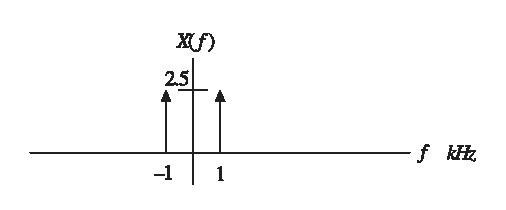
\includegraphics[width=\linewidth]{./img/img12}
        \end{figure}
    \end{itemize}
\end{frame}

\begin{frame}{Jawaban Latihan Soal 1}
    \begin{itemize}
        \item setelah analog signal di sampling dengan sampling rate 8000 Hz, maka sample signal spectrum dan kembarannya berada di frekuensi $\pm kf_s$ yang dengan scaled-amplitude sebesar $2.5/T$
        \begin{figure}
            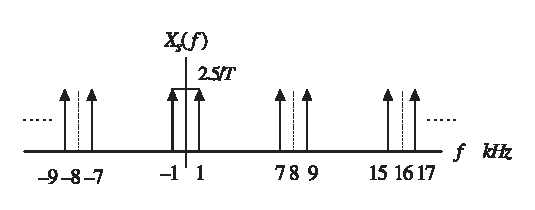
\includegraphics[width=\linewidth]{./img/img13}
        \end{figure}
    \end{itemize}
\end{frame}

\begin{frame}{Latihan Soal 2 dan 3}
    \begin{enumerate}
        \setcounter{enumi}{1}
        \item Diketahui analog signal
        \begin{equation*}
            x(t) = 5 \cos (2 \pi 1500 t),~\text{ untuk } t \geq 0
        \end{equation*}
        dan sampling rate sebesar 8 kHz.
        \begin{enumerate}
            \item[a.] Gambarkan spectrum dari original signal
            \item[b.] Gambarkan spectrum dari sampled signal dari 0 hingga 20 kHz
        \end{enumerate}
    
        \item Diketahui analog signal
        \begin{equation*}
            x(t) = 5 \cos (2 \pi 2500 t) + 2 \cos (2 \pi 3200 t),~\text{ untuk } t \geq 0
        \end{equation*}
        dan sampling rate sebesar 8 kHz.
        \begin{enumerate}
            \item[a.] Gambarkan spectrum dari original signal
            \item[b.] Gambarkan spectrum dari sampled signal dari 0 hingga 20 kHz
        \end{enumerate}
    \end{enumerate}
\end{frame}

\end{document}